
%%%%%%%%%%%%%%%%%%%%%%%%%%%%%%%%%%%%%%%%%
% University/School Laboratory Report
% LaTeX Template
% Version 3.1 (25/3/14)
%
% This template has been downloaded from:
% http:\\www.LaTeXTemplates.com
%
% Original author:
% Linux and Unix Users Group at Virginia Tech Wiki 
% (https:\\vtluug.org/wiki/Example_LaTeX_chem_lab_report)
%
% License:
% CC BY-NC-SA 3.0 (http:\\creativecommons.org/licenses/by-nc-sa/3.0/)
%
%%%%%%%%%%%%%%%%%%%%%%%%%%%%%%%%%%%%%%%%%

%----------------------------------------------------------------------------------------
%	PACKAGES AND DOCUMENT CONFIGURATIONS
%----------------------------------------------------------------------------------------

\documentclass[12pt]{article}
\usepackage{booktabs}
\usepackage{float}
\usepackage{fontspec}
\usepackage{mathtools}
\usepackage{xcolor}
\usepackage{titlesec}
%\usepackage{arial}
\usepackage{mathptmx}
\usepackage[version=3]{mhchem} % Package for chemical equation typesetting
\usepackage{siunitx} % Provides the \SI{}{} and \si{} command for typesetting SI units
\usepackage{graphicx} % Required for the inclusion of images
\usepackage{hyperref}
\usepackage{amsmath} % Required for some math elements 
\usepackage{inputenc}
\usepackage[T1]{fontenc}
%\usepackage[portuguese]{babel}
\usepackage{hyphenat}
\usepackage{helvet}
\usepackage{titlesec}
\usepackage{titling}
\usepackage{setspace}
\usepackage{booktabs}
\usepackage[acronym,nomain,nonumberlist,toc]{glossaries} % 
\usepackage[british,UKenglish,USenglish,american]{babel}

%\hyphenation{mate-mática recu-perar}

\usepackage{etoolbox}

\AtBeginDocument{%
	\setlength{\abovedisplayskip}{6pt}
	\setlength{\belowdisplayskip}{6pt}
}

\setcounter{tocdepth}{6}
\setcounter{secnumdepth}{6}



\makeatletter
\g@addto@macro\normalsize{%
	\setlength\abovedisplayskip{6pt}
	\setlength\belowdisplayskip{6pt}
	\setlength\abovedisplayshortskip{6pt}
	\setlength\belowdisplayshortskip{6pt}
}
\makeatother

\setlength\parindent{0pt} % Removes all indentation from paragraphs

\renewcommand{\labelenumi}{\alph{enumi}.} % Make numbering in the enumerate environment by letter rather than number (e.g. section 6)

\setsansfont{Arial}
% Set serifed font to Cambria
%\setmainfont{Times New Roman}
\setmainfont[SizeFeatures={Size=12}]{Arial}
\newfontfamily\subsubsectionfont{Times New Roman} %12pt large
\newfontfamily\headingfont[]{Arial}
% Set formats for each heading level
\titleformat*{\section}{\Large\bfseries\sffamily}
\titleformat*{\subsection}{\Large\bfseries\sffamily}
\titleformat*{\subsubsection}{\itshape\subsubsectionfont}

\font\myfon=Arial at 17pt
\font\myfont=Arial at 15pt
\font\myfontt=Arial at 12pt

\usepackage{enumitem}
\usepackage{booktabs}
\usepackage{graphicx}


\newfontfamily\capfont[SizeFeatures={Size=10}]{Times New Roman}
\newfontfamily\mathfont[SizeFeatures={Size=12}]{Times New Roman}


\usepackage{caption}
\DeclareCaptionFont{cap}{\capfont}

\makeatletter %only needed in preamble
\renewcommand\scriptsize{\@setfontsize\scriptsize{10pt}{10pt}}
\makeatother
\captionsetup{font=cap, labelfont=cap}

\usepackage{subcaption}
\usepackage{wrapfig}

\renewcommand{\thesection}{\Roman{section}.} 
\renewcommand{\thesubsection}{\thesection\Roman{subsection}}
\renewcommand{\baselinestretch}{1.5} 

\titlespacing*{\section}
{0pt}{6pt}{3pt}

\titlespacing*{\subsection}
{0pt}{6pt}{3pt}

\titlespacing*{\subsubsection}
{0pt}{6pt}{3pt}

%\setmainfont{mathptmx}

\usepackage{geometry}
\geometry{
	a4paper,
	total={170mm,257mm},
	left=20mm,
	top=20mm,
}


\usepackage{spverbatim}


\usepackage{listings}
\lstset{
	keywordstyle=\color{RoyalBlue},
	basicstyle=\small\ttfamily,
	commentstyle=\color{black}\ttfamily,
	%    rulecolor=\color{black},
	showstringspaces=false,
	breaklines=true,
	frameround=ftff,
	frame=single,
	columns=flexible,
	%    belowcaptionskip=5em,
	aboveskip=1.25em,
	language=Verilog,
}

\renewcommand{\lstlistingname}{Code excerpt} 

 \setlength{\belowcaptionskip}{-10pt}





\begin{document}
	
	
	%----------------------------------------------------------------------------------------------------------------------------------------------------------------------------------------------------
	%																					CAPA
	%----------------------------------------------------------------------------------------------------------------------------------------------------------------------------------------------------
	
	%----------------------------------------------------------------------------------------------------------------------------------------------------------------------------------------------------
	%----------------------------------------------------------------------------------------------------------------------------------------------------------------------------------------------------
	\begin{titlepage}
		\begin{figure}
			
\includegraphics[scale=0.4]{IST} 
		\end{figure}
		
		\vspace*{3cm}
		\begin{center}
			\headingfont\Large{\bfseries INSTITUTO SUPERIOR TÉCNICO}\\[2cm]
			\headingfont\LARGE{\bfseries Design Test and Reliability of Electronic Systems \\[1,5cm]Project 2 - Circular Bist}\\[0,5cm]
			%\headingfont\Large{\bfseries RELATÓRIO FORMAL}
		\end{center}
		\vspace{3cm}
		\headingfont\hfill
		\begin{tabular}{@{}l@{}}
		    Group 2\\ 
			n$^{\circ}$ 77973 - Pedro Pina\\
			n$^{\circ}$ 84779 - Afonso Muralha\\
			\\
			Professor Fernando Gonçalves
			
		\end{tabular}
		\vspace{2,5cm}
		\begin{center}
			\today
		\end{center}
	\end{titlepage}
	%----------------------------------------------------------------------------------------------------------------------------------------------------------------------------------------------------
	%																						CAPA
	%----------------------------------------------------------------------------------------------------------------------------------------------------------------------------------------------------
	\newpage

    \tableofcontents

	\newpage



	\section{Introduction and Objectives}
	The goal of this project is to develop a controller that fulfills certain specifications.\\
	The controller must be described in synthesizable Verilog and it must synthesize without any errors or warnings. \\
	To validate the quality of the testbench, the code coverage must be evaluated using the Cadence simulator (Xcelium).
	
	\section{Circular BIST design}
	The circular BIST system must be applied to a given circuit, different for each group. The circuit in question is named ''circuito06'' and its as follows: 
	\begin{figure}[!htb]
        \centering
        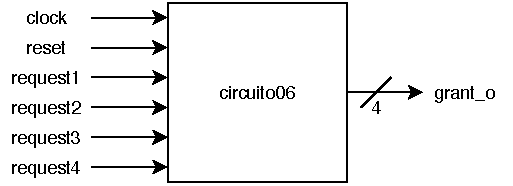
\includegraphics[scale=1]{circuito06.pdf}
            \caption{''circuito06'' interface.}
            \label{fig:ci}
    \end{figure}
    
    The implemented system has the following diagram:
    
    \begin{figure}[!htb]
        \centering
        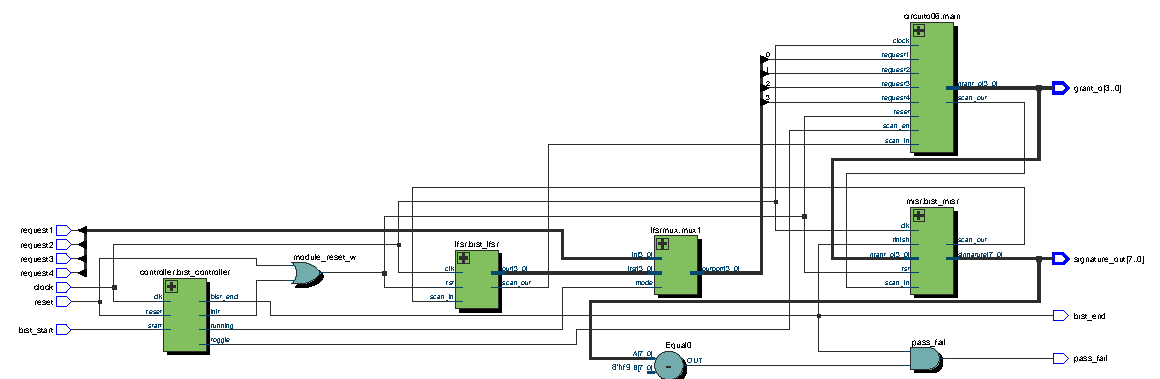
\includegraphics[scale=0.8]{block_diagram.pdf}
            \caption{Circular BIST block diagram.}
            \label{fig:bd}
    \end{figure}
    
    \subsection*{LFSR and MISR}
    
    In order to generate pseudo-random input for the circuit, an external linear feedback shift register was implemented. Since there are 4 inputs for the circuit, the LFSR features 4 flip-flop stages with XOR feedback on the forth and third flip-flops in order to make the output polynomial maximal-length:
    
    \begin{equation}
        \begin{matrix}
            \text{Polynomial} = x^{4} + x^{3} + 1 
            \\ 
            \text{Period}= 2^{4} -1 = 15
        \end{matrix}
    \end{equation}
    
    Finally, to make it scan compatible, the scan-in was added to the XOR chain. This adds another degree of randomness to the system and makes it more likely to find faults.
    Additionally a temporary seed input was added for testing purposes.
    
    The LFSR is represented in verilog:
  
    \begin{lstlisting}[caption={Counter variables.},captionpos=b]
module lfsr #
(   
    parameter NBIT = 4,
    parameter SEED = 4'b1111
) (
    input clk,
    input rst,
    input scan_in,
    // input [3:0] seed, //this is only used for testing
    output [NBIT-1:0] out,
    output scan_out
);

    reg [NBIT-1:0] dff;

    assign out[0] = dff[0];
    assign out[1] = dff[1];
    assign out[2] = dff[2];
    assign out[3] = dff[3];
    
    assign scan_out = dff[3];

    always @ (posedge clk) begin
        if(rst) begin
            dff <= SEED;
        end
        else begin
            dff <= {dff[4-2:0], dff[3] ^ dff[2] ^ scan_in};
        end
    end

endmodule
    \end{lstlisting}
    
    A test-bech was create to ensure the periodicity of the LFSR. The testbench is able to set a user determined seed and will cycle the LFSR until the output patterns repeats. When it does, the iteration number is printed and the program execution stops. In this case, the scan input is disabled.\\
    Test result:
        
        \begin{lstlisting}[caption={Counter variables.},captionpos=b]
linuxdev@linuxdev-VirtualBox:/media/sf_GitHub/PTFSE-Classes/Project2$ make lfsr_test
Initial seed:          15
LFSR output: 15
LFSR output: 14
LFSR output: 12
LFSR output:  8
LFSR output:  1
LFSR output:  2
LFSR output:  4
LFSR output:  9
LFSR output:  3
LFSR output:  6
LFSR output: 13
LFSR output: 10
LFSR output:  5
LFSR output: 11
LFSR output:  7
End in          15 iterations
Should be 2^4-1 =          15
    \end{lstlisting}
    
The output of the circuit is fed into an internal multiple input signature register. With this the input sequence of the MISR will generate a quasi-unique signature for a BIST cycle. The lengh chosen for the MISR was 8, but other sizes were tested, for example, 16. With 8 flip-flops the xor chain used in order to make output polynomial maximal-length was:
    
    \begin{equation}
            \text{Polynomial} = x^{8} + x^{6} x^{5} + x^{4} + 1 
    \end{equation}   
    
The LFSR is represented in verilog:
  
    \begin{lstlisting}[caption={Counter variables.},captionpos=b]
// `define misr16
`define misr8

module misr #
(
    `ifdef misr16
    parameter NBIT = 16
    `endif

    `ifdef misr8
    parameter NBIT = 8
    `endif
)(
    input clk,
    input rst,
    input scan_in,
    input[3:0] grant_o,
    input finish,
    output[NBIT-1:0] signature,
    output scan_out
);

    reg [NBIT-1:0] dff;

`ifdef misr16
<definition for 16 bit misr supressed>
`endif

`ifdef misr8

    assign signature = dff;
    assign scan_out = dff[7];

    parameter seed = 8'b11111111;

    always @ (posedge clk) begin
        if(rst) begin
            dff <= seed;
        end
            dff[0] <= grant_o[3] ^ dff[NBIT-1];          
            dff[1] <= grant_o[2] ^ dff[0];
            dff[2] <= grant_o[1] ^ dff[1] ^ dff[NBIT-1];
            dff[3] <= grant_o[0] ^ dff[2] ^ dff[NBIT-1];
            dff[4] <= scan_in    ^ dff[3] ^ dff[NBIT-1];
            dff[5] <=              dff[4];
            dff[6] <=              dff[5];
            dff[7] <=              dff[6];
        end
    end

`endif

endmodule
    \end{lstlisting}
    
To ensure that the MISR works correctly, two testbenches were created. Fist, like the LFSR the outputs of the MISR were read each cycle until it reached the first output. In this case all of the MISR inputs were set to zero. 
    
    \begin{lstlisting}[caption={Counter variables.},captionpos=b]
linuxdev@linuxdev-VirtualBox:/media/sf_GitHub/PTFSE-Classes/Project2$ make misr_test
Initial signature:         255
MISR output: 255
MISR output:  70
MISR output: 140
<output truncated>
MISR output: 229
MISR output: 215
MISR output: 179
MISR output: 123
MISR output: 246
MISR output: 241
End in         255 iterations
Should be 2^8-1 =         255
    \end{lstlisting}    
    
The second testbench   
    
    
    
    
    
	In order to add it to a circular BIST system, the circuit needs to be scan compatible.
    
    
    
 \newpage   
	
	\section{Conclusion}
	This project objective was to learn how to program and develop a controller with certain \mbox{specifications}. This meant that, for it to work properly, the ones developing it, needed to have a clear understanding of every input and ouput signals functionality and behaviour \mbox{- how} does a signal influences other signals and how does it develop throw a specific time period.\\ 
	Therefore, having tools such as the Gtkwave and the Cadence simulator (Xcelium) are important to evaluate the code, which errors and warnings it may have, during the developing stage. In addition to that, having a graphic representation of what has been done can guarantee that the final product is working as intended, with every specification running correctly.

	\begin{thebibliography}{20}
\bibitem{ref1}
Verilog Tutorial (Course slides)\\
\url{https://fenix.tecnico.ulisboa.pt/downloadFile/1126518382240212/My%20Verilog%20Tutorial.pdf}

\end{thebibliography}


\end{document}
